
% ----------------------------------------------------------------------
%                   LATEX TEMPLATE FOR PhD THESIS
% ----------------------------------------------------------------------

% based on Harish Bhanderi's PhD/MPhil template, then Uni Cambridge
% http://www-h.eng.cam.ac.uk/help/tpl/textprocessing/ThesisStyle/
% corrected and extended in 2007 by Jakob Suckale, then MPI-CBG PhD programme
% and made available through OpenWetWare.org - the free biology wiki


%: Style file for Latex
% Most style definitions are in the external file PhDthesisPSnPDF.
% In this template package, it can be found in ./Latex/Classes/
\documentclass[twoside,11pt]{Latex/Classes/PhDthesisPSnPDF}


%: Macro file for Latex
% Macros help you summarise frequently repeated Latex commands.
% Here, they are placed in an external file /Latex/Macros/MacroFile1.tex
% An macro that you may use frequently is the figuremacro (see introduction.tex)
% This file contains macros that can be called up from connected TeX files
% It helps to summarise repeated code, e.g. figure insertion (see below).

% insert a centered figure with caption and description
% parameters 1:filename, 2:title, 3:description and label
\newcommand{\figuremacro}[3]{
	\begin{figure}[htbp]
		\centering
		\includegraphics[width=1\textwidth]{#1}
		\caption[#2]{\textbf{#2} - #3}
		\label{#1}
	\end{figure}
}

% insert a centered figure with caption and description AND WIDTH
% parameters 1:filename, 2:title, 3:description and label, 4: textwidth
% textwidth 1 means as text, 0.5 means half the width of the text
\newcommand{\figuremacroW}[4]{
	\begin{figure}[htbp]
		\centering
		\includegraphics[width=#4\textwidth]{#1}
		\caption[#2]{\textbf{#2} - #3}
		\label{#1}
	\end{figure}
}

% inserts a figure with wrapped around text; only suitable for NARROW figs
% o is for outside on a double paged document; others: l, r, i(inside)
% text and figure will each be half of the document width
% note: long captions often crash with adjacent content; take care
% in general: above 2 macro produce more reliable layout
\newcommand{\figuremacroN}[3]{
	\begin{wrapfigure}{o}{0.5\textwidth}
		\centering
		\includegraphics[width=0.48\textwidth]{#1}
		\caption[#2]{{\small\textbf{#2} - #3}}
		\label{#1}
	\end{wrapfigure}
}

% predefined commands by Harish
\newcommand{\PdfPsText}[2]{
  \ifpdf
     #1
  \else
     #2
  \fi
}

\newcommand{\IncludeGraphicsH}[3]{
  \PdfPsText{\includegraphics[height=#2]{#1}}{\includegraphics[bb = #3, height=#2]{#1}}
}

\newcommand{\IncludeGraphicsW}[3]{
  \PdfPsText{\includegraphics[width=#2]{#1}}{\includegraphics[bb = #3, width=#2]{#1}}
}

\newcommand{\InsertFig}[3]{
  \begin{figure}[!htbp]
    \begin{center}
      \leavevmode
      #1
      \caption{#2}
      \label{#3}
    \end{center}
  \end{figure}
}


%%% Local Variables: 
%%% mode: latex
%%% TeX-master: "~/Documents/LaTeX/CUEDThesisPSnPDF/thesis"
%%% End: 

\usepackage[T1]{fontenc}
\usepackage{array}
\usepackage{pdfpages}

\usepackage{adjustbox}
\usepackage{algorithmic}
\usepackage{amsmath,amssymb,amsfonts}
%\usepackage[backend=bibtex,style=ieee]{biblatex}
%\usepackage{bookmark}
\usepackage{tabularx,array}
\usepackage{booktabs}
\usepackage{caption}
% \usepackage{cite}
\usepackage{color}
\usepackage[inline]{enumitem}
\usepackage{float}
\usepackage[T1]{fontenc}
%\usepackage{fontspec}
\usepackage{svg}
\usepackage{footnote}
\usepackage{graphicx}
% \usepackage[colorlinks=true,citecolor=blue]{hyperref}
% \usepackage{inputenc}[utf8]
\usepackage{listings}
% \usepackage{textcomp}
\usepackage[flushleft]{threeparttable}
% \usepackage{subcaption}
\usepackage{xcolor}
\usepackage{cleveref}

%\usepackage{graphics}
% or use the graphicx package for more complicated commands
%\usepackage{graphicx}

% ------------------------------------------------------------------------%
% Proper Python Syntax Highlighting                                       %
% Author: redmode
% https://tex.stackexchange.com/questions/83882/how-to-highlight-python   %
% -syntax-in-latex-listings-lstinputlistings-command#83883                %
% ----------------------------------------------------------------------- %

% Default fixed font does not support bold face
\DeclareFixedFont{\ttb}{T1}{txtt}{bx}{n}{8} % for bold
\DeclareFixedFont{\ttm}{T1}{txtt}{m}{n}{8}  % for normal

% Custom colors
\definecolor{deepblue}{rgb}{0,0,0.5}
\definecolor{deepred}{rgb}{0.6,0,0}
\definecolor{deepgreen}{rgb}{0,0.5,0}

% Python style for highlighting
\newcommand\pythonstyle{
	\lstset{
		language=Python,
		basicstyle=\ttm,
		showstringspaces=false,
		tabsize=4,
		aboveskip=0.2cm,
		belowskip=0.2cm,
		otherkeywords={self},             % Add keywords here
		keywordstyle=\ttb\color{deepblue},
		emph={MyClass,__init__},          % Custom highlighting
		emphstyle=\ttb\color{deepred},    % Custom highlighting style
		stringstyle=\color{deepgreen},
		frame=tb,                          % Any extra options here
		prebreak=\textbackslash,
		linewidth=8.85cm,
		breaklines=true,
	}
}

% Python environment
\lstnewenvironment{python}[1][] {
	\pythonstyle\lstset{#1}
}{}

% Python for inline
\newcommand\pythoninline[1]{{\pythonstyle\lstinline!#1!}}

% Python for external file
\newcommand\pythonexternal[2][]{{\pythonstyle\lstinputlisting[#1]{#2}}}

% ----------------------------------------------------------------------- %

% Bash style for highlighting
\newcommand\bashstyle{
	\lstset{
		language=Bash,
		basicstyle=\ttm,
		showstringspaces=false,
		tabsize=2,
		%commentstyle=itshape,
		aboveskip=0.2cm,
		belowskip=0.2cm,
		prebreak=\textbackslash,
		extendedchars=true,
		mathescape=false,
		% literate= {\$}{{\textcolor{blue}{\$}}}1 {&}{{\textcolor{blue}{\&}}}1 {/n}{{\textcolor{green}{\textbackslash n}}}1,
		linewidth=8.85cm,
		breaklines=true
	}
}

% Bash environment
\lstnewenvironment{bash}[1][] {
	\bashstyle\lstset{#1}
}{}

% Bash for inline
\newcommand\bashinline[1]{{\bashstyle\lstinline!#1!}}

% Bash for external file
\newcommand\bashexternal[2][]{{\bashstyle\lstinputlisting[#1]{#2}}}


% Python style for highlighting
\newcommand\cstyle{
	\lstset{
		language=c,
		basicstyle=\ttm,
		showstringspaces=false,
		tabsize=4,
		aboveskip=0.2cm,
		belowskip=0.2cm,
		otherkeywords={self},             % Add keywords here
		keywordstyle=\ttb\color{deepblue},
		emph={MyClass,__init__},          % Custom highlighting
		emphstyle=\ttb\color{deepred},    % Custom highlighting style
		stringstyle=\color{deepgreen},
		frame=tb,                          % Any extra options here
		prebreak=\textbackslash,
		linewidth=8.85cm,
		breaklines=true,
	}
}

% Python environment
\lstnewenvironment{clist}[1][] {
	\cstyle\lstset{#1}
}{}

% Python for inline
\newcommand\cinline[1]{{\cstyle\lstinline!#1!}}

% Python for external file
\newcommand\cexternal[2][]{{\cstyle\lstinputlisting[#1]{#2}}}

% ----------------------------------------------------------------------- %

%: ----------------------------------------------------------------------
%:                  TITLE PAGE: name, degree,..
% ----------------------------------------------------------------------
\usepackage{graphicx}

      \textwidth 15cm
      \textheight 22cm
      \parindent 10pt
      \oddsidemargin 0.85cm
      \evensidemargin 0.37cm


\begin{document}

\thispagestyle{empty}

\begin{center}

Vrije Universiteit Amsterdam \hspace*{2cm} Universiteit van Amsterdam

\vspace{1mm}

\hspace*{-7.5cm}\includegraphics[height=25mm]{0_frontmatter/figures/vu-griffioen.pdf}

\vspace*{-2cm}\hspace*{7.5cm}\includegraphics[height=15mm]{0_frontmatter/figures/uva_logo.jpg}

\vspace{2cm}

{\Large Master Thesis}

\vspace*{1.5cm}

\rule{.9\linewidth}{.6pt}\\[0.4cm]
{\huge \bfseries OpenCSD: Log-Structured Filesystem enabled Computational
Storage Device platform\par}\vspace{0.4cm}
\rule{.9\linewidth}{.6pt}\\[1.5cm]

\vspace*{2mm}

{\Large
\begin{tabular}{l}
{\bf Author:} ~~Corne Lukken ~~~~ (2639319)
\end{tabular}
}

\vspace*{2cm}

\begin{tabular}{ll}
{\it 1st supervisor:}   & ~~Animesh Trivedi \\
{\it daily supervisor:} & ~~Animesh Trivedi \\
{\it 2nd reader:}       & ~~supervisor name
\end{tabular}

\vspace*{2.5cm}

\textit{A thesis submitted in fulfillment of the requirements for\\ the joint UvA-VU Master of Science degree in Computer Science}

\vspace*{1.8cm}

\today\\[4cm] % Date

\end{center}

\newpage


% ----------------------------------------------------------------------
       
% turn off those nasty overfull and underfull hboxes
\hbadness=10000
\hfuzz=50pt


%: --------------------------------------------------------------
%:                  FRONT MATTER: dedications, abstract,..
% --------------------------------------------------------------


%\language{english}


% sets line spacing
\renewcommand\baselinestretch{1.2}
\baselineskip=18pt plus1pt


%: ----------------------- generate cover page ------------------------

\begin{center}
\textit{``Software engineers are often one of the last lines of defense against potentially dangerous and unethical practices'' \\ from {\em The code I’m still ashamed of}, by Bill Sourour (2015)}
\end{center}

%: ----------------------- cover page back side ------------------------
% Your research institution may require reviewer names, etc.
% This cover back side is required by Dresden Med Fac; uncomment if needed.

\newpage
%\vspace{10mm}
%1. First Reader: Name Surname
%
%\vspace{10mm}
%2. Daily Supervisor: Name Surname
%
%\vspace{10mm}
%3. Second Reader: Name Surname
%
%\vspace{10mm}
%4. Industrial Supervisor: Name Surname
%
%\vspace{20mm}
%Day of the defense:

%\vspace{20mm}
%\hspace{70mm}Signature from head of PhD committee:



%: ----------------------- abstract ------------------------

% Your institution may have specific regulations if you need an abstract and where it is to be placed in the document. The default here is just after title.


% Thesis Abstract -----------------------------------------------------


%\begin{abstractslong}    %uncommenting this line, gives a different abstract heading
\begin{abstracts}        %this creates the heading for the abstract page

Here goes the abstract of this thesis.
\end{abstracts}
%\end{abstractlongs}


% ---------------------------------------------------------------------- 


% The original template provides and abstractseparate environment, if your institution requires them to be separate. I think it's easier to print the abstract from the complete thesis by restricting printing to the relevant page.
% \begin{abstractseparate}
%   
% Thesis Abstract -----------------------------------------------------


%\begin{abstractslong}    %uncommenting this line, gives a different abstract heading
\begin{abstracts}        %this creates the heading for the abstract page

Here goes the abstract of this thesis.
\end{abstracts}
%\end{abstractlongs}


% ---------------------------------------------------------------------- 

% \end{abstractseparate}


%: ----------------------- tie in front matter ------------------------

\frontmatter
% Thesis Dedication ---------------------------------------------------

%\begin{dedication} %this creates the heading for the dedication page

%To ...

%\end{dedication}

% ----------------------------------------------------------------------
% Thesis Acknowledgements ------------------------------------------------


% \begin{acknowledgementslong} %uncommenting this line, gives a different acknowledgements heading
% \begin{acknowledgements}      %this creates the heading for the acknowlegments

% If you find this thesis hard to read, filled with to much whitespace or
% otherwise prefer a more dense layout, an alternative version is available 
% online:

% \end{acknowledgements}
% \end{acknowledgmentslong}

% ------------------------------------------------------------------------





%: ----------------------- contents ------------------------

\setcounter{secnumdepth}{3} % organisational level that receives a numbers
\setcounter{tocdepth}{3}    % print table of contents for level 3
\tableofcontents            % print the table of contents
% levels are: 0 - chapter, 1 - section, 2 - subsection, 3 - subsection


%: ----------------------- list of figures/tables ------------------------

\listoffigures	% print list of figures

\listoftables  % print list of tables




%: ----------------------- glossary ------------------------

% Tie in external source file for definitions: /0_frontmatter/glossary.tex
% Glossary entries can also be defined in the main text. See glossary.tex
% 
% this file is called up by thesis.tex
% content in this file will be fed into the main document

% Glossary entries are defined with the command \nomenclature{1}{2}
% 1 = Entry name, e.g. abbreviation; 2 = Explanation
% You can place all explanations in this separate file or declare them in the middle of the text. Either way they will be collected in the glossary.

% required to print nomenclature name to page header
% \markboth{\MakeUppercase{\nomname}}{\MakeUppercase{\nomname}}


% ----------------------- contents from here ------------------------

\newlength{\nomenlabelindent}
\setlength{\nomenlabelindent}{13em}
\newenvironment{nomenclature2}{%
\newcommand\entry[2]{%
   \hangindent\nomenlabelindent\noindent\makebox[\nomenlabelindent][l]{##1\quad}\ignorespaces##2\par}%
   \addcontentsline{toc}{chapter}{\protect\numberline{}Glossary}%
   \section*{Glossary}}{\par\addvspace{12pt}}

\begin{nomenclature2}
    \entry{HDD}{Hard-Disk Drive} % 233
    \entry{SSD}{Solid-State Drive} % 234
    \entry{NVMe}{Non-Volatile Memory express} % 250
    \entry{FTL}{Flash Translation Layer} % 255
    \entry{CSx}{Computational Storage Device} % 257
    \entry{ISA}{Instruction Set Architecture} % 274
    \entry{eBPF}{extended Berkely Packet Filter} %293
    \entry{ZNS}{Zoned NameSpaces} % 294
    \entry{Host Managed}{Storage device that performs no automatic garbage
        collection or wear leveling exposing facilities to do so to the host} % 296
    \entry{Hybrid Filesystem}{Filesystem supporting both regular access as well
        as Computational Storage offloading} % 296
    \entry{LFS}{Log-Structured Filesystem} % 297
    \entry{FPGA}{Field-Programmable Gate Array} % 306
    \entry{PCIe}{Peripheral Component Interconnect express} % 310
    \entry{OS}{Operating System} % 324
    \entry{VFS}{Virtual FileSystem} % 326
    \entry{FUSE}{Filesystem in USErspace} % 327
    \entry{GPGPU}{General-Purpose computing on Graphics Processing Units} % introduction 149
    \entry{API}{Application Programming Interface} % introduction 150
    \entry{ABI}{Application Binary Interface} % introduction 159
    \entry{NAT}{Node Address Table} % 406
    \entry{OCSSD}{Open-Channel SSD} % relatedwork 29
    \entry{Programming Model}{See our previous survey
        \textit{Past, Present and Future of Computational Storage: A Survey} chapter 8.2 \cite{lukken2021past}} % relatedwork 48
    \entry{Degree of Programmability}{See our previous survey
        \textit{Past, Present and Future of Computational Storage: A Survey} chapter 8.2 \cite{lukken2021past}} % relatedwork 51
    \entry{RPC}{Remote Procedure Call} % relatedwork 57
    \entry{HTTP}{HyperText Transfer Protocol} % relatedwork 57
    \entry{SQL}{Structured Query Language} % relatedwork 96
    \entry{CSEE}{Computational Storage Execution Environment} % relatedwork 64
    \entry{SIT}{Segment Info Table} % relatedwork 64
    \entry{SSA}{Segment Summary Area} % relatedwork 64
    \entry{RTL}{Register-Transfer Level} % relatedwork 127
    \entry{NVMe-oF}{NVMe over Fabrics} % relatedwork 184
    \entry{MPI}{Message Passing Interface} % relatedwork 145
    \entry{HPC}{High-Performance Computing} % relatedwork 146
    \entry{CS}{Computer Science} % relatedwork 231
    \entry{POSIX}{Portable Operating System Interface} % design 101
    \entry{NIX}{A UNIX based operating system or derivative} % design 110
    \entry{PID}{Process IDentifier} % design 115
    \entry{Kernel}{Compiled binary or bytecode representation of a computational
        unit that can be submitted / scheduled for execution on accelarator type
        devices such as graphics cards or CSxs. Alternatively, resource and
        device management layer of an operating system.} % implementation 89
    \entry{EOF}{End Of File} % implementation 841
\end{nomenclature2}

% \printnomenclature

%\nomenclature{LSY}{ehbfuefebbfbjkjkebfjbfbfw} 
%\nomenclature{DEPC}{diethyl-pyro-carbonate; used to remove RNA-degrading enzymes (RNAases) from water and laboratory utensils}
%\nomenclature{DMSO}{dimethyl sulfoxide; organic solvent, readily passes through skin, cryoprotectant in cell culture}
%\nomenclature{EDTA}{Ethylene-diamine-tetraacetic acid; a chelating (two-pronged) molecule used to sequester most divalent (or trivalent) metal ions, such as calcium (Ca$^{2+}$) and magnesium (Mg$^{2+}$), copper (Cu$^{2+}$), or iron (Fe$^{2+}$ / Fe$^{3+}$)}
 

\begin{multicols}{2} % \begin{multicols}{#columns}[header text][space]
\begin{footnotesize} % scriptsize(7) < footnotesize(8) < small (9) < normal (10)

\printnomenclature[1.5cm] % [] = distance between entry and description
\label{nom} % target name for links to glossary

\end{footnotesize}
\end{multicols}



%: --------------------------------------------------------------
%:                  MAIN DOCUMENT SECTION
% --------------------------------------------------------------

% the main text starts here with the introduction, 1st chapter,...
\mainmatter

\renewcommand{\chaptername}{} % uncomment to print only "1" not "Chapter 1"


%: ----------------------- subdocuments ------------------------

% Parts of the thesis are included below. Rename the files as required.
% But take care that the paths match. You can also change the order of appearance by moving the include commands.


% this file is called up by thesis.tex
% content in this file will be fed into the main document

%: ----------------------- introduction file header -----------------------
\chapter{Introduction}

% the code below specifies where the figures are stored
\ifpdf
    \graphicspath{{1_introduction/figures/PNG/}{1_introduction/figures/PDF/}{1_introduction/figures/}}
\else
    \graphicspath{{1_introduction/figures/EPS/}{1_introduction/figures/}}
\fi

% ----------------------------------------------------------------------
%: ----------------------- introduction content ----------------------- 
% ----------------------------------------------------------------------



%: ----------------------- HELP: latex document organisation
% the commands below help you to subdivide and organise your thesis
%    \chapter{}       = level 1, top level
%    \section{}       = level 2
%    \subsection{}    = level 3
%    \subsubsection{} = level 4
% note that everything after the percentage sign is hidden from output



\section{Context} 

% We have a separate previous work section we will ignore most of the different
% related literature in the introduction.

% Problem

The amount of data being generated and processed worldwide is growing rapidly.
Meanwhile the prevelant Von Nuemann computer architecture requires all data is 
moved to system memory before it can be processed \cite{2018-neumann-bottleneck}.
Until recently storage devices such as hard-disk drives (HDDs) or solid state
drives (SSDs) have only been passively storing data. With the increasing
bandwidth persistent storage devices like SSDs achieve this excessive data
movement to memory is increasingly becoming a bottleneck \cite{2014-micro-ndp}.
Similarly, the CPU generational performance
improvements \cite{2016-western-digital} as well as link speeds of interconnects
are stagnating compared to nand flash bandwidth \cite{10.1145/3286588}, the
underlying technology enabling modern SSDs.

% Potential solution and benefits

A promising solution to this problem is the processing of data in-situ by
pushing compute to the storage layer. This solution is actively being researched
as \textit{"Programmable Storage"} and \textit{"Computational Storage"} among
other terms. The concept is not new however, as it has been previously
explored in database mainframes \cite{database-computer} as well as for
conventional HDDs \cite{active-disk-pillar, active-disks-tech,
intelligent-disk}. With rise of Non-Volatile Memory Express (NVMe) technologies
offering signifcantly more device-internal bandwidth this concept is being
revisted. What makes NVMe SSDs even more suited is that they already contain
capable processing units often boasting even multiple cores. This requirement
comes from the internal management the device has to perform known as the
\textit{Flash Translation Layer} (FTL). Devices utilizing computational elements
on conventional SSDs for \textit{Computational Storage} are commonly known as
\textit{Computational Storage Devices} (CSx)s. The potential benefits of such a
heteregenous architecture offering programmable storage include energy saving,
cost reduction and performance improvements.

% Challenges

Despite all these benefits there is still no widespread adoption even after a
decade of research \cite{lukken2021past}. A multitude of challenges
have prohibited this adoption of which several still applicable today. Four
prominent challenges include that, firstly, \textit{Computational Storage}
requires complete vertical integration. Meaning that changes are required at all
levels of abstraction, device hardware, interfaces, drivers and operating system
to name a few. Trying to integrate a solution for all levels in one prototype
results in a very large problem space. This large problem space complicates
deriving standards for designs and interfaces although the development of such a
standard by SNIA is on-going \cite{snia-model}. Secondly, vendors might choose
to use different hardware with different
\textit{Instruction Set Architectures} (ISA)s or different host-to-device
interfaces. These differences might result in incompatible user applications
across vendors hurting reusability and hindering adoption. Third, filesystems
are managed by the host operating system while the FTL is
managed by the device. Given that one is not aware of the processes within the
other, this semantic gap complicates several aspects such as consistency,
concurreny, multi-user tenancy and filesystem integration. Lastly, no
specialized filesystem designs exist that support both regular user access
concurrent with \textit{Computational Storage} offloading.

% Solutions

In this work we address each of these challenges directly and propose a
complete \textit{Computational Storage} solution that offers a filesystem
capable of concurrent multi-user tenancy with both regular and compute
offloading access (hybrid). We introduce each of the solutions briefly before
describing their complete case. Firstly, we circumvent the complexity of
complete vertical integration by creating a simulation platform on top of
QEMU \cite{qemu}. Secondly, We eliminate potential incompatibities across vendors
by using \textit{Extended Berkely Packet Filer} (eBPF) \cite{what-ebpf} as
compute kernel language. Third, We bridge the semantic gap by using Zoned
Namespaces (ZNS) \cite{zns} SSDs which moves the FTL to the host operating
system (host-managed). Lastly, we allow for concurrent multi-user tenancy in
a \textit{Hybrid Filesystem} context by developing a specialized
\textit{Log-Structured Filesystem} (LFS) \cite{Rosenblum1992TheDA} with an
in-memory snapshot consistency model \cite{Viotti2016ConsistencyIN}. We present
this complete solution as \textit{OpenCSD} an open-source Apache 2 licensed CSx
simulation framework with accompanying filesystem called
FluffleFS \cite{qemu-csd}.

\subsection*{A Case for CSx Simulation}

The lack of a standardized design has lead to a large variety of different
hardware architectures being explored including using embedded CPUs or
\textit{Field-Programmable Gate Arrays} (FPGA)s. Moreover, closed-source
devices have even become commercially available. Still there is a lot of
uncertainty about the right computational hardware models, interconnects and
interconnects their interfaces. Even though the \textit{Peripheral Component
Interconnect Express} (PCIe) interconnect and the NVMe storage interface
currently dominate modern storage devices it is unclear if their current
capabilities are sufficient to support CSxs. Meanwhile existing technologies
such as QEMU allow rapid development of new simulated hardware.

The lack of a clear standardized design combined with the ease of prototyping
designs in simulation clearly shows that choosing simulation over an actual
hardware prototype is the current logical choice.

\subsection*{A Case for eBPF Programmability}

The concept of programmability provides end users the capability to run their
own provided code. With the introduction of modern \textit{Operating Systems}
(OS)s this is expected to happen in safe and dynamic manner. Programmability
can be achieved in different manners such as through the kernel in kernel
modules, with filesystems through \textit{Virtual File System} (VFS) or FUSE and
with language runtimes such as those in Python. In addition programmability can
also target a peripheral instead of the host directly such as is prevelant in
\textit{General-Purpose computing on Graphics Processing Units} (GPGPU)
programming through \textit{Application Programming Interfaces} (API)s like
OpenCL \cite{opencl} and CUDA \cite{cuda}. Through similar mechanisms
programmability in CSxs can be achieved.

The uncertainty of the hardware design makes it unclear exactly how close to the
hardware and through which method of programmability CSxs will be effective.
Although, naturally, the closer to the actual storage the better
(Near-Data Processing). Therefor, our programmability must not be restricted or
favor a particular type.

Introducing eBPF an ISA and API with a large collection of toolchains and
wideranging implementations \cite{what-ebpf, McCanne1993TheBP}. These
implementations range from complex such as the one found in the Linux kernel to
simple such as the one found in uBPF \cite{ubpf}, with the key difference in
complexity being the supported API. Effectively, the implementation running
(runtime) eBPF code decides the API by tying special eBPF syscall instructions
to predefined code. In addition, this allows the user program and runtime to
exchange important information such as prominently done in Linux through eBPF
maps \cite{bpf-man}.

The benefits of eBPF are four fold. First, the ISA is not tailored to any
specific domain and it has been used in networking \cite{xdp},
tracing \cite{enhanced-ebpf} and security \cite{seccomp} applications. Second,
the simple nature of the eBPF ISA allows for verification and bounded execution
checking such as performed by the Linux kernel \cite{kern-analysis}. Third, eBPF
supports efficient code generation through jitting achieving close to bare-metal
performance. Lastly, eBPF has been positioned as the unified ISA for
heteregenous computing \cite{Brunella2020hXDPES, bpf-uapi}.

\subsection*{A Case for ZNS}

A new emerging NVMe standard is Zoned Namedspaces (ZNS). It can been seen as the
technical successor to Open-Channel % \cite{}.
This standard allows host visibility and control over data placement
(host-managed) while more closely representing nand flash behavior. This
replacement for the traditional block interface offers reduced
write-ampplifcation, lower SSD hardware requirements and more intelligent
wear-leveling and garbage collection. However ZNS SSDs come with several
constraints such as not allowing in-place updates (append-only), using a large
collection of sectors as single erasure unit and requiring wear-leveling and
garbage collection to be explicitly programmed by the host.

Yet we argue ZNS greatly improves the feasibility of CSx supporting
\textit{hybrid filesystems}. Firstly, ZNS offers more predictable performance in
conjuction with \textit{Log-Structured Filesystems} as the absence of an FTL
means the behavior of \textit{append-only} writes won't be influenced by
underlying write-amplification or garbage-collection. Secondly, the direct
relationship between dimensions as reported to the host and to those known on
the device results in a greatly simplified exchange of information from host
submitted compute kernels as well as reduced kernel runtime translations.
Finally, this reduced semantic gap between the host and device is essential to
compute kernels running autonomously and without shared virtual memory.

\subsection*{A Case for LFS}

\textit{Log-Structured Filesystems} have been around for a long
time \cite{Rosenblum1992TheDA} but have not really been popularized until the
recent advancement of nand flash. A LFS maintains one or multiple logs which
are append-only sections of the filesystem. This has the advantage of the
underlying device receiving filesystem writes as sequential I/O operations,
which is known to improve performance. In addition, LFSs are often relatively
easy to implement. Unfortunately, LFSs suffer from write-amplification because
modifcations updating inode or other data location information travels up the
chain in history.

Yet we argue an LFS is essential for an effective \textit{hybrid filesystem} due
to the following three reasons. Firstly, the append-only nature of a LFS is the
best fit for the append-only requirement of ZNS SSDs. Secondly, the
chronological order of logs allow for snapshotting, versioning and simplified
crash recovery. It is thanks to the properties of an LFS that FluffleFS is able
to provide in-memory snapshots to compute kernels. Lastly, the problem around
write-amplification is a solved issue thanks to the F2FS \cite{Lee2015F2FSAN}
work which introduced so called Node Address Tables (NAT).

\section{Research Question}

How to achieve multi-user tenancy in a Log Structured Filesystem (LFS) while
supporting Computational Storage offloading?

\subsection{Sub Questions}

What would a Zoned Namespaces (ZNS) Log Structured Filesystem (LFS) look like?

How to register Computational Storage Device (CSx) compute kernels using
existing operating system APIs?

How to differentiate individual users, files and I/O operations in relation to
their CSx compute kernel?

\section{Research Method}

%  Iterative design approach


% this file is called up by thesis.tex
% content in this file will be fed into the main document

\chapter{Related Work} % top level followed by section, subsection


% ----------------------- paths to graphics ------------------------

% change according to folder and file names
\ifpdf
    \graphicspath{{7/figures/PNG/}{7/figures/PDF/}{7/figures/}}
\else
    \graphicspath{{7/figures/EPS/}{7/figures/}}
\fi


% ----------------------- contents from here ------------------------
% 

\section{Support Technologies}

Several developments across different fields have been essential for the
goals we envision for CSx. In this section we go to the most prominent of 
these developments. However, only developments not directly related to CSxs are
covered as the next section covers these CSx developments in detail.

These developments are three fold. Firstly, the development of host-managed
storage interfaces with first \textit{Open-Channel SSD} (OCSSD)
\cite{Bjrling2017LightNVMTL} and later NVMe ZNS. Secondly, filesystem
improvements with F2FS \cite{Lee2015F2FSAN} using an optimized layout for flash
storage devices. Lastly, a heterogenous compute ISA, namely eBPF
\cite{ebpf_cs_2021, kourtis2020safe, bpf-uapi}.

OCSSD exposes the flash layout through an end user API \cite{liblightnvm}.
Effectively, this moved the FTL with wear-leveling and gargabe collection
functionality to the host. However, the intricate details of this flash layout
made the API hard to use for users as well as implement for SSD vendors. In
addition, vendors might fear that exposing all these details could leak trade
secrets. A more succesful alternative to OCSSD is NVMe ZNS which is now a
ratified extension to the NVMe specification \cite{nvme-zns}. In NVMe ZNS the
flash layout is exposed in zones. Subsequently, all sectors in a zone must be
written in a sequentially incremented fashion as well as the entire zone must
be erased as a whole. Finally, ZNS devices can impose limits on the maximum
amount of zones that can be opened at any given time. This zoned layout is
visually compared to a conventional flash SSD in figure \ref{figure:znslayout}.

\begin{figure}[H]
    \centering
	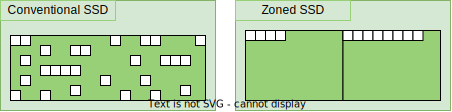
\includegraphics[width=0.8\textwidth]{resources/images/zns-vs-conventional-layout.pdf}
	\caption{Comparison of conventional and ZNS SSD data layouts}
    \label{figure:znslayout}
\end{figure}

This new ZNS technology has already been used in promising research avenues such
as an optimized garbage collection scheme \cite{254268}. In addition, we see
a more general performance evaluations \cite{10.1145/3458336.3465300, 9188086}
demonstrating the advantages of ZNS. Lastly, we see proposals to extend the ZNS
interface to better support compaction in LFSs \cite{273709}.

% Transition sentence?

It is only recently that we have seen filesystems optimized for flash outside of
embedded applications. This new filesystem, F2FS \cite{Lee2015F2FSAN}, is
significantly more advanced than embedded filesystem like JFFS2 \cite{jffs2}.
With F2FS write-amplification is not only prevented by utilizing the sequential
write behavior of LFSs, in addition, it is prevented by tracking inode locations
in a separate NAT as oppossed to chaining inode location data together. This
flattened layout solves the wandering tree problem where a single location
updates causes a chain of updates to propagate. Other improvements include
separate logs for hot and cold data as well as garbage collection using a
\textit{Segment Info Table} (SIT) and \textit{Segment Summary Area} (SSA).
However, F2FS still has several limitations such as no wear-leveling and only
entirely invalidated zone garbage-collection. An overview of the F2FS data
layout is shown in figure \ref{figure:f2fslayout}.

\begin{figure}[H]
    \centering
	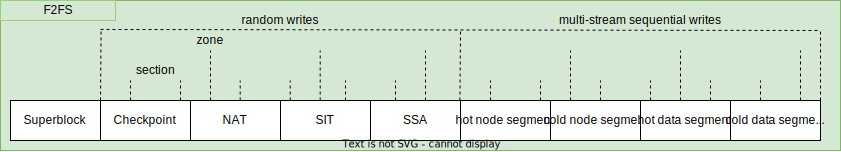
\includegraphics[width=1\textwidth]{resources/images/f2fs-layout.png}
	\caption{Overview of data layout on F2FS}
    \label{figure:f2fslayout}
\end{figure}

% Transition sentence?

eBPF is used in the Linux kernel extensively and is still seeing increasing use
cases. One of these recent new use cases is as heterogenous ISA \cite{bpf-uapi}.
The combination of the ease of virtualization together with the call instruction
enables to separate an API from its actual implementation. Even more, the
implementation is so separated from its implementation that it does not have to
be linked at compile time or even be present on the host system. Previous works
have already explained why eBPF is such a good fit for computational storage in
detail \cite{ebpf_cs_2021}. Lastly, the capabilities of eBPF have already been
demonstrated in the case of disaggregated storage \cite{kourtis2020safe}.

\section{Computational Storage Devices}

While OpenCSD is unique it is by no means the first CSx prototype as there
has been over a decade of research in this field \cite{lukken2021past}. In this
decade we have seen a large variety of approaches, problem spaces, hardware
platforms and software APIs. There is significant progression in this field, 
however, several important challenges are still open research
questions \cite{barbalacecomputational}.

In this section we introduce characteristics of CSx prototypes, the most
prominent open research questions, provide an overview of notable works,
describe the progression of the field and describe fundamentally missing
features that hinder adoption and widespread use of CSxs.

% Introduce early working prototypes

% Demonstrate different hardware platforms, embedded CPU, vs FPGA.

% List of BPF using storage literature (Blockndp:, Extos: Data-centric
%extensible os, Ex-tension framework for file systems in user space, 
%  Safe and efficient remote application code execu-tion on disaggregated NVM,
% BPF for storage: an exokernel-inspired approach )

% Introduce previous ZCSD table but extended

\subsection{CSx characterstics}

There are four types of characteristics that set CSxs apart. First there is
the end user \textit{programming model}, the model of programming developers
have to use in order to interact with CSx. Second, there is the execution
environment, the level of software abstraction the end user programs are run on
(on the device). Third, is the \textit{degree of programmability}, the amount of
programming control offered to the end user. Lastly, there is the interface used
to connect the device to the host.

With end user programming models there are, in no particular order,
\textit{Dataflow (MapReduce, DAG)}, \textit{Client / Server
(RPC \footnotemark[1], HTTP \footnotemark[2])}, \textit{Shared memory} and
\textit{Declarative (Regex, MySQL)}. Although simple categories, the correct
attribution of these categories can become quite complicated due to nuances. For
instance, if an end user needs to link to a new shared library to call methods
with MySQL queries as argument it becomes unclear what the programming model
should be. In this work we argue \textit{Shared memory} as the library that
needs to be linked is introduced in the work.

\footnotetext[1]{\textit{Remote Procedure Call} (RPC)}

\footnotetext[2]{\textit{HyperText Transfer Protocol} (HTTP)}

In \textit{Computational Storage Execution Environments} (CSEE) we effectively
observe seven distinct levels of abstraction. These range from
\textit{Register-Transfer Level} (RTL) design such as using languages like
Verilog or VHDL to virtual machines. The compiled output of RTL designs is known
as a bitstream and typically programmed into an FPGA at runtime. The distinct
levels are listed below.

\begin{enumerate}
    \item Bistream; bitstream programmed directly unto FPGA.
    \item Embedded; single program, single memory space, no OS just 'real mode'.
    \item Accelerators; OpenCL, Vulkan.
    \item Real-Time operating system;
    \item Operating System;
    \item Container;
    \item Virtual Machine;
\end{enumerate}

We see a similarly large range in different \textit{degrees of programmability}
from no end user programmability at all such as with transparent operations to
arbitrary code execution. The six distinct levels are shown below. It
should be noted, howerver, that the first two levels can be regarded as no or a
lack of end user programmability.

\begin{enumerate}
    \item Transparent operations, (de)compression (Playstation 5 I/O Controller)
    \item Fixed functions, unchangeable, workload specific \cite{2013-fast-active-flash}
    \item Fixed function dataflow programming \cite{Wickremesinghe02distributedcomputing}
    \item Query offloading, SQL\footnotemark[3], NoSql, Regex \cite{10.14778/2994509.2994512}
    \item Event driven (hooks) user-programmable functions \cite{10.1145/3429357.3430519}
    \item Arbitrary code execution, VHDL, eBPF, TCL \cite{10.1145/605432.605425, kourtis2020safe}
\end{enumerate}

\footnotetext[3]{\textit{Structured Query Language} (SQL)}

It is important to illustrate that the \textit{degree of programmability} is
fundamentally different from the end user \textit{programming model} as one
denotes how programs are submitted and run on the device while the other denotes
what model an end user must use to develop for the CSx respectively.

\subsection{Past CSx Works}

Using these characteristics of CSxs allows to make a qualitative comparison of
different works from the past decade. By arranging all these works in
publication order as shown in table \ref{table:csxoverview} we can start to
obeserve developments in the field. We describe three different types of
observations being general observations, observations relating to changes over
time and finally observations on specific works.

Firstly, we can observe that the amount of works with a limited \textit{degree
of programmability} is small, consisting of just \textit{Active Flash
\cite{active-flash-piller, 2013-fast-active-flash},
Caribou \cite{10.14778/3137628.3137632}, LeapIO \cite{10.1145/3373376.3378531}
and CSD 2000 \cite{10.1145/3399666.3399934}}. Additionally, there is substantial
diversity between each work but the use of event driven programmability, shared
memory programming model, PCIe interface and either bitstream or embedded
execution environments stand out. Although not necessarily in combination with
one another. There is also a strong correlation between the client / server
programming model and operating system execution environment. Most of the works
utilizing this combination achieve this with either \textit{NVMe over Fabrics}
(NVMe-oF) or NVMe over TCP.

Secondly, the main change over time is related to the shift from SATA to PCIe
NVMe interfaces. Less pronounced changes include a slight shift to more
arbitrary code execution programmability and a shift away from an embedded
execution environment. Not shown in table \ref{table:csxoverview} is the
transition to more complex and more complete prototypes. These changes include
trying to address challenges related to security, usability and filesystem
support. However, the extend of how these challenges are addressed remains
limited particularly regarding filesystem support \cite{barbalacecomputational}.
One of the most recent works BlockNDP \cite{10.1145/3429357.3430519} was
designed for supporting regular filesystem access but it is clear that it is
still missing in the prototype, for instance\footnotemark[4]. The most complete
is Metal FS \cite{10.1145/3342195.3387557} which achieves filesystem integrated
computational offloading through UNIX pipes. However, it does not address
multi-user tenancy. In addition, it is unclear if their customized Unix pipe
behaviour influences regular UNIX pipes should they be used on their filesystem.

\footnotetext[4]{"Support for accessing a file on a file system could be added,
for example, by integrating it with a FUSE file system driver or uNFS"
\cite{10.1145/3429357.3430519}}

Several specific developments of individual works are of interest. Firstly,
NGD newport \cite{10.1145/3415580} manages to support different programming
models by offering SSH access to the CSx. While novel we do not see this model
work for widespread adoption because of the barrier to entry in programming for
distributed systems as opposed to heterogenous architectures. This can be
partially overcome by offering an API on the host at the expense of the
flexibility to choose the programming model. Secondly, Catalina
\cite{8855540} utilizes the \textit{Message Passing Interface} (MPI), an
industry leading standard library in \textit{High-Performance Computing} (HPC),
to achieve distributed memory parallelization. However, this suffers from the
same drawback as NGD newport of HPC being a larger barrier to entree compared to
the use of accelerators such as GPGPU in heterogenous architectures. Third,
is Cognitive SSD \cite{8839401} which utilizes accelerator type interfaces such
as OpenCL to achieve programmability. Although in the complete architecture we
think this interface is essential it should be hidden from the end users. In
this work we will demonstrate that this can be achieved through filesystem
extended attributes (xattr). Lastly, Metal FS \cite{10.1145/3342195.3387557}
is interesting because it is the only work to use the relatively new CAPI
cache coherent interface \cite{Stuecheli2015CAPIAC}, in addition to, 
integrating filesystem support using FUSE and UNIX pipes. Finally, Metal FS
comes with both a C and C++ library which obfuscate the underlying use of pipes
to improve usability.

\begin{table}
    \caption{Related CSx works from the past decade}
    \centering
    \begin{adjustbox}{width=1\textwidth}
        \begin{threeparttable}[]
            \begin{tabular}{lllll}
                \toprule
                \textbf{Name} & \textbf{Programmability} & \textbf{Programming Model} & \textbf{Interface} & \textbf{CSEE} \\
                \midrule
                Active SSD \cite{6062973} & Event driven & Dataflow (streams) & PCIe & Operating system (Custom) \\
                Active Flash \cite{active-flash-piller, 2013-fast-active-flash} & Fixed functions & N.A. & SATA (OpenSSD) & Embedded \\
                Smart SSD \cite{6558444} & Event driven & Dataflow (MapReduce) & SATA & Embedded \\
                Smart SSD \cite{10.1145/2463676.2465295} & Event driven & Shared memory & SATA & Embedded \\
                Intelligent SSD \cite{10.1145/2464996.2465003, 10.1145/2505515.2507847} & Arbitrary code execution\footnotemark[5] & Shared memory\footnotemark[5] & N.A. & Operating system (Linux)\footnotemark[5] \\
                Ibex \cite{10.14778/2732967.2732972} & Query offloading (MySQL) & Declarative & SATA & Bitstream \\
                Willow \cite{186149} & Arbitrary code execution & Client / Server (RPC) & PCIe (NVMe) & Operating system (Custom) \\
                Biscuit \cite{2016-isca-biscuit} & Event driven & Dataflow & PCIe & Embedded \\
                Hadoop ISC* \cite{7524716} & Event driven & Dataflow (MapReduce) & SAS & Embedded \\
                YourSQL \cite{10.14778/2994509.2994512} & Query offloading (MySQL) & Declarative & PCIe (NVMe) & Bitsream\footnotemark[6] \\
                Caribou \cite{10.14778/3137628.3137632} & Fixed functions (key-value store) & Client / Server (RPC) & Ethernet & Bitstream \\
                Summarizer \cite{10.1145/3123939.3124553} & Event driven & Shared memory & PCIe (NVMe) & Embedded \\
                NDP RE2 regex* \cite{10.1145/3211922.3211926} & Query offloading (Regex) & N.A. & N.A. & Embedded \\
                Registor \cite{10.1145/3310149} & Query offloading (Regex) & Shared memory & PCIe (NVMe) & Bitsream \\
                Cognitive SSD \cite{8839401} & Arbitrary code execution & Shared memory & PCIe (NVMe, OpenSSD) & Accelerators (Custom) \\
                INSIDER \cite{234968} & Event driven & Shared memory (VFS) & PCIe & Bitstream \\
                Catalina \cite{8855540} & Arbitrary code execution & Client / Server (MPI) & PCIe (NVMe) & Operating system (Linux) \\
                LeapIO \cite{10.1145/3373376.3378531} & Fixed functions & Transparent & Ethernet (RDMA) & Embedded \\
                THRIFTY \cite{10.1145/3400302.3415723} & Event driven\footnotemark[7] & Shared memory (VFS)\footnotemark[7] & PCIe\footnotemark[7] & Bitstream\footnotemark[7] \\
                POLARDB \cite{246154} & Query offloading (POLARDB) & Declarative & PCIe & Bitstream \\
                NGD newport \cite{10.1145/3415580} & Arbitrary code execution & Client / Server & PCIe (NVMe) & Operating system (Linux) \\
                CSD 2000 \cite{10.1145/3399666.3399934} & Fixed functions (compression) & Transparent & PCIe (NVMe) & Bitstream \\
                Metal FS \cite{10.1145/3342195.3387557} & Event driven & Dataflow (streams) & PCIe (NVMe) \/ CAPI & Bitstream \\
                blockNDP \cite{10.1145/3429357.3430519} & Event driven & Dataflow (streams) & PCIe (NVMe, OpenSSD) & Virtual Machine (QEMU) \\
                QEMU CSD \cite{10.1145/3439839.3459085} & Arbitrary code execution & Shared memory & PCIe (NVMe) & N.A. (Simulated) \\
                ZCSD \cite{lukken2021zcsd} & Arbitrary code execution & Shared memory & N.A. (Simulated) & Virtual Machine (uBPF) \\
                \bottomrule
            \end{tabular}
            \begin{tablenotes}[para,flushleft]
                \centering Overview of CSx works and the previously elaborated
                characteristics.
            \end{tablenotes}
        \end{threeparttable}
        \label{table:csxoverview}
    \end{adjustbox}
\end{table}

\footnotetext[5]{Simulations performed by porting workloads unto ARM based
processor. No actual hardware on SSDs is used.}

\footnotetext[6]{The work uses special FCPs with hardware based filtering
functions. We assume these must be implemented using FPGAs although the work
does not specify.}

\footnotetext[7]{Build on top of the INSIDER software stack.}

\subsection{Reproducibility}

In science the ability to reproduce a work and verify its claims is essential.
Moreover, it might be the verify cornerstone of the scientific method. However,
in \textit{Computer Science} (CS) many works fundamentally rely on software and
hardware prototypes while the source code or design files are never published.
Reproducibility of a work introducing new software or hardware without these
related files is practically impossible!

This problem of unreproducible works and unverifiable claims is prevelant
throughout the works relating to CSxs. Out of the 27 referenced works only four
\cite{10.14778/3137628.3137632, 234968, 8839401, lukken2021zcsd}
\footnotemark[8] of them have released source code. While only one has released
the hardware design files (VHDL) \cite{10.14778/3137628.3137632}. The result is
that 85 percent of these works are very likely unreproducible and their claims
unverifiable. We believe that any work introducing hardware or software should
release the related files or be rejected for publication!

Clearly there have been substantial developments in several technologies related
to CSx as well as in CSx research itself. However, proper design requirements
are needed in order to adress any of the remaining open research questions.

\footnotetext[8]{The author of BlockNDP\cite{10.1145/3429357.3430519} has also
been trying to release the source code ever since October 2020 but is likely
facing severe holdback from Huawei. It is unclear if the source code will ever
be released.}

% ---------------------------------------------------------------------------
% ----------------------- end of thesis sub-document ------------------------
% ---------------------------------------------------------------------------

% this file is called up by thesis.tex
% content in this file will be fed into the main document

\chapter{Design} % top level followed by section, subsection


% ----------------------- paths to graphics ------------------------

% change according to folder and file names
\ifpdf
    \graphicspath{{7/figures/PNG/}{7/figures/PDF/}{7/figures/}}
\else
    \graphicspath{{7/figures/EPS/}{7/figures/}}
\fi


% ----------------------- contents from here ------------------------
% 

\section{Requirements}

\subsection{Framework}

% mmap shared memory vs monolith (iteration 1)
% accelerator API vs NVMe namespace (iteration 4)

\subsection{Filesystem}

% rtl_next vs FUSE (iteration 3)

% Two write pointers, one for RANDOM ZONE and one for LOG ZONE. Use of ZNS is
% optional but allows for lower write-amplification and more explicit garbage
% collection

\subsubsection{Concurrency}

\subsection{Offloading}

% Filesystem extended attributes, PID + INODE

\section{Iterations}

Before covering our overall design decisions we describe the iterations that
have occured during the design process. We cover this separately as to not
clutter the overall design and implementation sections. These next sections
describes the design requirements derived from the research questions, followed
by, the final design. The implementation details of the design are covered in
a subsequent chapter.

The overall design process consisted of four destinct iterations. Two relating
primarily to the framework, onr relating to the filesystem and one relating to
offloading. This section describes each iteration briefly before going in more
detail. Firstly regarding framework iterations we see the distinct decision
to switch from a multi process architecture using mmap for shared memory maps to
a monolithic application. The second iteration led to switching away from the
design of an accelerator API, much like Vulkan or OpenCL, to an artificial
extension of the NVMe namespace. The third iteration changed the use
rtld\_next \cite{rtldnext} to using a practical filesystem with FUSE. Lastly, as
computational storage API our work switched from using
\textit{Portable Operating System Interface} (POSIX) fadvise \cite{fadvise} to
extended attributes.

For each of these four iterations the advantages of the change as well as the
major issues with the previous solution are described. Each iteration is
described in the same order as previously defined.

\subsection{Shared Memory Monolith}

Modern operating systems offer fastly different methods to write sofware. From
kernel modules, to distributed processes, UNIX pipes and shared memory maps.
Choosing the right model impacts practicalities such as the amount of
development effort required and the robustness of the final solution. 
Furtermore, depending on the software architecture some solutions will be better
suited than others.

During the design the use of shared memory maps was replaced with using regular
shared memory. While both solutions provide shared memory they are fundamentally
different. A shared memory map is a file, leveraging the well known UNIX
principle \textit{everything is a file}, that allows two or more processes to
share a region of memory. While regular shared memory is limited to a single
process although it could share this memory with additional threads.

this single process shared memory solution is one of the most common found in
software today. The concepts of such a program are very well understood as
well as the development using imperative languages being straightforward.

While shared memory maps are typically found in device drivers, such as those
for graphics cards, their use consistutes severe additional development effort.
In conjuction with our design being a simulation there is no scientific value in
using shared memory maps for our design.

\subsection{NVMe Namespace Command Set}

\subsection{FUSE Filesystem}

\subsection{Extended Attributes}

% ---------------------------------------------------------------------------
% ----------------------- end of thesis sub-document ------------------------
% ---------------------------------------------------------------------------

% this file is called up by thesis.tex
% content in this file will be fed into the main document

\chapter{Implementation} % top level followed by section, subsection


% ----------------------- paths to graphics ------------------------

% change according to folder and file names
\ifpdf
    \graphicspath{{7/figures/PNG/}{7/figures/PDF/}{7/figures/}}
\else
    \graphicspath{{7/figures/EPS/}{7/figures/}}
\fi

\section{OpenCSD}

In this section we describe the tools and techniques used with the OpenCSD
framework, detail modules with their respective functionality and show the
external dependencies as well as internal relationships of these modules. 
Followed by, sections on filesystem and offloading implementation details.

\subsection{Framework}

Firstly, OpenCSD consist of many external dependencies, most prominently
\textit{Storage Performance Development Kit} (SPDK) \cite{spdk} and uBPF
\cite{ubpf}. These technolgies are used as userspace NVMe SSD driver and as
virtual machine for the eBPF ISA respectively. Reusing as many as pre-existing
technologies as possible increases the change of familiarity aiding ease of use.
More prominently, these existing technologies dramatically lower the amount of
development effort required to create the prototype. However, our design
requirements demand these dependencies be installed in an isolated way. To do
this OpenCSD configures an isolated build environment with dependencies made
available through an environment file. Moreover, this file configures variables
such as \textit{PATH} and \textit{LD\_LIBRARY\_PATH}. In addition, OpenCSD
offers a QEMU installation and accompanying qcow image to emulate a ZNS SSDs.
This is to overcome the limited availability of these SSDs as stated in the
design requirements. However, the use of QEMU for ZNS SSDs is entirely optional.
Finally, CMake \cite{cmake} is used to orchestrate the installation of
dependencies as well as the compilation of binary targets. Due to limitations it
is advised to rerun CMake after each make command, as this  prevents unnecessary
recompilation of external dependencies \footnotemark[9]. The combination of this
isolated dependencies environment managed through CMake with the ability to use
QEMU for ZNS SSDs emulation is ideal to minimize the complexity as exposed to
users of OpenCSD.

\footnotetext[9]{Due to limitations in the evaluation of file presence
conditions which are not reevaluated when executing the generated makefile.}

As said OpenCSD is comprised of modules using a component architecture.
Additionally, Each module is compiled as a static or shared library to reduce
coupling. This creates an explicit nature of exchanging information between
linked libraries that allows to identify feasibility problems at an early stage.
This is opposed to potentially only identifying such issues when creating a
first hardware prototype. A trivial example of such infeasibilities would be
using shared memory mutexes to synchronize filesystem and CSx kernel behaviour.
Several modules are solely an interface with subsequent modules being one or
more concrete implemenations of these interfaces. These module based interfaces
with loose coupling allow for simplified replacement of technologies.

\subsubsection{Modules}

The overall modules of OpenCSD are shown in figure
\ref{figure:moduledependencies} along with any external or internal
dependencies. In addition, we briefly describe the functionality of each module.
Finally, at the end of this subsection we describe the three most prominent
modules of OpenCSD.

% Diagram with overview of different modules and their used as well as
% relationships. Also show integration of open-source technologies.

\begin{figure}
    \centering
	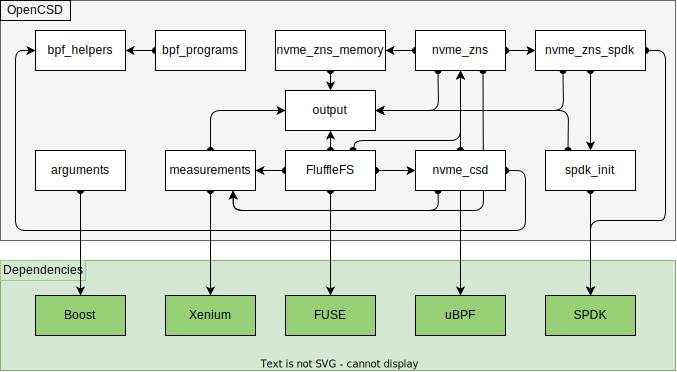
\includegraphics[width=1\textwidth]{resources/images/module-dependencies.pdf}
	\caption{Overview of all OpenCSD components and their depends-on relations}
    % \includesvg[width=0.6\columnwidth]{resources/images/module-dependencies}
    \label{figure:moduledependencies}
\end{figure}

\begin{itemize}
    \item output - Manages stdout and stderr output to the console by
    registering namespaces and providing a variety of log levels.
    \item arguments - Parses command line arguments and splits these into parts
    that can be passed to other modules in a decoupled nature. 
    \item measurements - Low overhead performance instrumentation for functions
    separated by namespaces using high performance lockless unbounded queue
    \cite{Michael1996SimpleFA}.
    \item spdk\_init - Collection of helpers to perform SPDK initialization and
    select ZNS suppporting NVMe namespace.
    \item nvme\_zns - NVMe interface to perform ZNS operations read, write and
    reset. To be used by FluffleFS for decoupled I/O operations.
    \item nvme\_zns\_memory - Memory backed implementation of nvme\_zns
    interface.
    \item nvme\_zns\_spdk - SPDK backed implementation of nvme\_zns interface
    \item nvme\_csd - Simulated extension to the PCIe NVMe protocol that allows
    to perform CSx operations. Execution of kernels is handled through uBPF.
    Utilizes instance of nvme\_zns to perform actual I/O operations performed by
    kernel.
    \item bpf\_helpers - Collection of headers that define the eBPF ABI
    supported for CSx kernels. ABI to be implemented by device vendor
    or in this case nvme\_csd for simulation. The ABI is filesystem agnostic.
    \item bpf\_programs - Collection of eBPF programs linked at runtime for
    previous ZCSD \cite{lukken2021zcsd} prototype.
    \item FluffleFs - FUSE LFS supporting in-memory snapshots to achieve
    multi-user tenancy with concurrent regular and offloaded filesystem access.
    Utilizes, nvme\_zns and nvme\_csd to achieve functionality.
\end{itemize}

Out of these components nvme\_csd, bpf\_helpers and FluffleFS are the most
essential. They simulate the required changes that would realize such an
architecture.

In short nvme\_csd contains functions that should be made part of a new NVMe
command set and namespace \cite{nvme-command} similar to how ZNS was introduced.
Currently, the functions are overly simplified so there is no use of the actual
command layout as well as lack of queue submissions and completion commands. We
feel the concepts of implementing these are well understood and would not
contribute to the scientific value of this work while introducing substantial
additional complexity.

bpf\_helpers contains the ABI exposed to the eBPF kernels. An ABI is different
from an API in that the functions it defines cannot be found in segments of
code, either included statically or through a shared library. Instead it uses
an ISA specific instruction that can be called with a set of arguments, the
arguments matching the function signature. Alternatively, should the ISA not
have a specific \textit{call} instruction, interrupt requests can be used to
achieve the same functionality. Upon calling the control flow is returned to
the operating system or in our case uBPF where the functions behavior is
implemented. The result is that an ABI allows to define functionality with
vendor agnostic implementations, similar to POSIX for operating systems. It
should be noted that ISAs typically have a hard limit on the number of arguments
that can be supported, in the case of eBPF this is five arguments. Lastly, is
FluffleFS which is described in the next section in detail.

Out of all modules only nvme\_zns has been given an abstract interface so the
underlying technologies can be easily replaced. However, we argue the design
requirements are still met as there are virtually no replacements for
technologies used in other modules such as uBPF and FUSE\footnotemark[10].
In addition, we feel it would have beneign benefits to create abstract
interfaces of the C++ STL. Our solution allows for replacing technologies with
readily available alternatives without creating unnecessary interfaces.

\footnotetext[10]{While alternative technolgies to implement filesystems exist
none of them are in userspace. As a result we argue there is no alternative to
FUSE.}

\subsection{Filesystem}

% Two write pointers, one for RANDOM ZONE and one for LOG ZONE. Use of ZNS is
% optional but allows for lower write-amplification and more explicit garbage
% collection

\subsubsection{Concurrency}

\subsection{Offloading}

% Filesystem extended attributes, PID + INODE

\section{Iterations}

This section is covered separetely to prevent clutter in the overall design and
implementation sections. This process consisted of four destinct iterations.
Two relating primarily to the framework, one to the filesystem and one to
offloading. This section describes each iteration briefly before going in more
detail. Firstly regarding framework iterations we see the distinct decision
to switch from a multi process architecture using mmap for shared memory maps to
a monolithic application. The second iteration lead to switching away from the
design of an accelerator API, much like Vulkan or OpenCL, to an artificial
extension of the NVMe namespace. The third iteration changed the use
rtld\_next \cite{rtldnext} to using a practical filesystem with FUSE. Lastly, as
computational storage API our work switched from using
\textit{Portable Operating System Interface} (POSIX) fadvise \cite{fadvise} to
extended attributes.

For each of these four iterations the advantages of the change as well as the
major issues with the previous solution are described. Each iteration is
described in the same order as previously defined.

\subsection{Shared Memory Monolith}

Modern operating systems offer fastly different methods to write sofware. From
kernel modules, to distributed processes, UNIX pipes and shared memory maps.
Choosing the right model impacts practicalities such as the amount of
development effort required and the robustness of the final solution. 
Furtermore, depending on the software architecture some solutions will be better
suited than others.

During the design the use of shared memory maps was replaced with using regular
shared memory. While both solutions provide shared memory they are fundamentally
different. A shared memory map is a file, leveraging the well known UNIX
principle \textit{everything is a file}, that allows two or more processes to
share a region of memory. While regular shared memory is limited to a single
process although it could share this memory with additional threads.

this single process shared memory solution is one of the most common found in
software today. The concepts of such a program are very well understood as
well as the development using imperative languages being straightforward.

While shared memory maps are typically found in device drivers, such as those
for graphics cards, their use consistutes severe additional development effort.
In conjuction with our design being a simulation there is no scientific value in
using shared memory maps for our design.

\subsection{NVMe Namespace Command Set}

\subsection{FUSE Filesystem}

\subsection{Extended Attributes}

% ---------------------------------------------------------------------------
% ----------------------- end of thesis sub-document ------------------------
% ---------------------------------------------------------------------------

% this file is called up by thesis.tex
% content in this file will be fed into the main document

\chapter{Consideration} % top level followed by section, subsection


% ----------------------- paths to graphics ------------------------

% change according to folder and file names
\ifpdf
    \graphicspath{{7/figures/PNG/}{7/figures/PDF/}{7/figures/}}
\else
    \graphicspath{{7/figures/EPS/}{7/figures/}}
\fi


\section{Design for Manufacter}

% The current prototype is only suitable for simulation. Several changes are
% necessary for real world applications. Firstly, addition to the NVMe command set
% in the form of a new NVMe namespace. Secondly, the ABI needs to be formalized
% and become a integral part of the specification. Third, existing drivers, such
% as SPDK or xNVME, must be updated to support this new namespace and commands.

% Describe how the design would change for a real world, practical
% implementation. Take the ICD loader diagram as base.

\begin{figure}
    \centering
	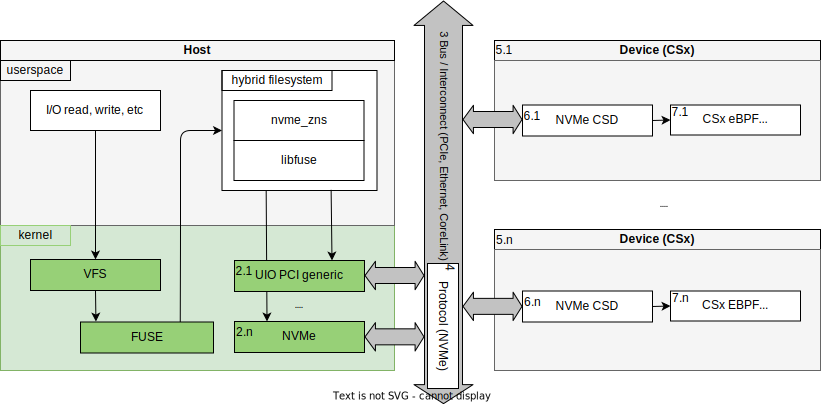
\includegraphics[width=1\textwidth]{resources/images/loader-pfs-arch-v3.png}
	\caption{Practical complete architecture for vendor agnostic CSxs with
        potential filesystem support.}
    % \includesvg[width=0.6\columnwidth]{resources/images/module-dependencies}
    \label{figure:practicalarchitecture}
\end{figure}

% Use statfs to determine the type of filesystem, ICDs are related to a specific
% filesystem type. The CSx eBPF ABI should contain atleast one system call to
% retrieve the vendor filesystem context data for the current request (already
% part of prototype). The CSx FS API contains functions and datastructures to
% allow the kernel to transform this context data. The API is implemented by
% individual filesystems as shared library and made available throught the ICD.
% The CSx FS runtime uses a loader with mechanisms such as \textit{dlopen} to
% verify the contents of the provided library in accordance to the API.

% The basic format of the ICD can be extended such that it could support
% extensions to the base API as well as contain versioning. Typically, ICD files
% are human readable using a markup language such as YAML. This is same approach
% as the prominent video graphics API Vulkan.

\begin{figure}
    \centering
	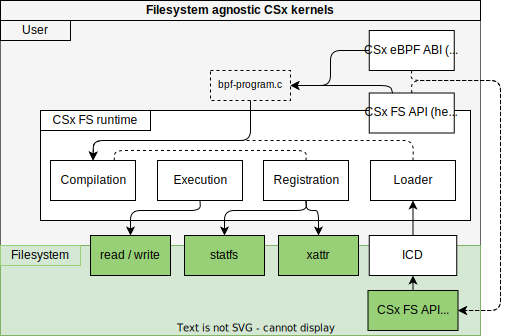
\includegraphics[width=0.7\textwidth]{resources/images/csx-fs-agnostic.png}
	\caption{Extended architecture to support filesystem agnostic CSx kernels.}
    % \includesvg[width=0.6\columnwidth]{resources/images/module-dependencies}
    \label{figure:csxfsruntime}
\end{figure}


% ---------------------------------------------------------------------------
% ----------------------- end of thesis sub-document ------------------------
% ---------------------------------------------------------------------------

\include{6_analysis/analysis}

\chapter{Results}

This section describes the results from the previously defined experiments.
Similar to the experiments section these results are separated into two
categories being microbenchmarks and applications.

For each result we explain the information being presented as well as further
findings. In addition, probably causes are discussed as well as
potential future experiments to investigate these claims.

\section{Microbenchmarks}

Several of the results for microbenchmarks are grouped together such as
sequential read and write results. Furtermore, all microbenchmark results use
linegraphs scaled with $log4$ on the horizontal axis. Using this scaling the
distance between different file and request sizes is proportional to their
difference in size. 

\begin{figure}
    \centering
	\includegraphics[width=1\textwidth]{resources/images/results-sequential.pdf}
	\caption{Results Sequential}
    % \includesvg[width=0.6\columnwidth]{resources/images/module-dependencies}
    \label{figure:moduledependencies}
\end{figure}

\begin{figure}
    \centering
	\includegraphics[width=1\textwidth]{resources/images/results-sequential-write.pdf}
	\caption{Results Sequential Write}
    % \includesvg[width=0.6\columnwidth]{resources/images/module-dependencies}
    \label{figure:moduledependencies}
\end{figure}

\begin{figure}
    \centering
	\includegraphics[width=1\textwidth]{resources/images/results-random-write.pdf}
	\caption{Results Sequential Write}
    % \includesvg[width=0.6\columnwidth]{resources/images/module-dependencies}
    \label{figure:moduledependencies}
\end{figure}

\begin{figure}
    \centering
	\includegraphics[width=1\textwidth]{resources/images/results-passthrough.pdf}
	\caption{Results Sequential Passthrough}
    % \includesvg[width=0.6\columnwidth]{resources/images/module-dependencies}
    \label{figure:moduledependencies}
\end{figure}


% Poor performance partially caused by FUSE, http://libfuse.github.io/doxygen/fast17-vangoor.pdf
% Especially 

\section{Shannon Entropy}

\begin{figure}
    \centering
	\includegraphics[width=1\textwidth]{resources/images/results-shannon-lower.pdf}
	\caption{Results Sequential Write}
    % \includesvg[width=0.6\columnwidth]{resources/images/module-dependencies}
    \label{figure:moduledependencies}
\end{figure}

\begin{figure}
    \centering
	\includegraphics[width=1\textwidth]{resources/images/results-shannon-upper.pdf}
	\caption{Results Sequential Passthrough}
    % \includesvg[width=0.6\columnwidth]{resources/images/module-dependencies}
    \label{figure:moduledependencies}
\end{figure}

% ---------------------------------------------------------------------------
% ----------------------- end of thesis sub-document ------------------------
% ---------------------------------------------------------------------------

\include{8_discussions/discussions}

\chapter{Conclusion}

To conclude, we have demonstrated that many previous prototype for flash based
CSxs exist and have been developed in the past decade. Until now, none of
these prototype where able to provide concurrent regular and offloaded
filesystem access, aptly named \textit{hybrid filesystems}. Our simulation
framework \textit{OpenCSD} and filesystem \textit{FluffleFS} are able to perform
offloading entirely using existing APIs, no shared libraries or network
communication is necessary. In addition, our kernels are vendor agnostic and
filesystem aware. Finally, our prototype runs entirely in userspace requiring no
understanding of the Linux kernel or modifications.

To do this our offloading is triggered through filesystem extended attributes
resulting in complete isolation from regular operating system behavior. These
filesystem extended attributes are present in all modern operating systems
including Windows, MacOs, FreeBSD and Linux. Across all previous CSx works only
a single other work managed to use existing APIs and in doing so they changed
UNIX pipe behavior \cite{10.1145/3342195.3387557}.

Concurrent regular and offloaded access is achieved by utilizing snapshot
consistency with LFS and ZNS technologies. Furthermore,
by utilizing eBPF and uBPF these kernels written for offloading can be made
vendor and filesystem agnostic. While the API for kernel filesystem support
still needs to be formalized and the proposed CSx runtime is still absent in our
prototype, the possibility of filesystem awareness in a concurrent regular and
offloaded setting has been proven. Furthermore we have proven that regular and
offloaded accesses can be easily differentiated utilized PID inode pairs.

Throughout this work we have argued why LFS, ZNS, eBPF and extended attributes
are the current best suited technologies to implement a hybrid filesystem.

We believe that many CSx prototype suffer from a high barrier to entree due to
complicated setup and technologies. Therefor, our design focussed heavily on
being easy to use to reduce barrier to entree. Our design has achieved this by
only utilizing userspace technologies, requiring no knowledge of kernel
development or any kernel modifications. In addition, our framework
\textit{OpenCSD} utilizes a component architecture that easily allows for
replacement of used technologies.

During the evaluation we showed that offloaded applications can reduce
data movement between the device and host by 99.9\% as well as drastically
reduce the host CPU load. However, the overall performance of FluffleFS still
needs to be improved significantly, only able to perform on par with flash
optimized filesystems under very select circumstances. Furthermore, our
limited performance optimizations made us unable to proof that concurrent
offloaded and regular file access can achieve unstagnated performance.

We encourage everyone to try our prototype today which is readily available
and open-source published under a permissive license \cite{qemu-csd}. Along our
source code are datasets of our measurements as well as the scripts to perform
these measurements and generate accompanying graphs. Even the source files for
this very thesis are included. We hope this openness inspires others to do the
same.

% ---------------------------------------------------------------------------
% ----------------------- end of thesis sub-document ------------------------
% ---------------------------------------------------------------------------
          
% this file is called up by thesis.tex
% content in this file will be fed into the main document

%: ----------------------- name of chapter  -------------------------
\chapter*{Appendix} % top level followed by section, subsection


%: ----------------------- paths to graphics ------------------------

% change according to folder and file names
\ifpdf
    \graphicspath{{X/figures/PNG/}{X/figures/PDF/}{X/figures/}}
\else
    \graphicspath{{X/figures/EPS/}{X/figures/}}
\fi

%: ----------------------- contents from here ------------------------
% \includepdf[pages=1-5]{CodesTable}
% \includepdf[pages=1-4]{InterviewQuestions}





% ---------------------------------------------------------------------------
%: ----------------------- end of thesis sub-document ------------------------
% ---------------------------------------------------------------------------


      
            
% --------------------------------------------------------------
%:                  BACK MATTER: appendices, refs,..
% --------------------------------------------------------------

% the back matter: appendix and references close the thesis


%: ----------------------- bibliography ------------------------

% The section below defines how references are listed and formatted
% The default below is 2 columns, small font, complete author names.
% Entries are also linked back to the page number in the text and to external URL if provided in the BibTex file.

% PhDbiblio-url2 = names small caps, title bold & hyperlinked, link to page 
%\begin{multicols}{2} % \begin{multicols}{ # columns}[ header text][ space]
%\begin{tiny} % tiny(5) < scriptsize(7) < footnotesize(8) < small (9)

\bibliographystyle{Latex/Classes/PhDbiblio-url2} % Title is link if provided
\renewcommand{\bibname}{References} % changes the header; default: Bibliography

\bibliography{11_references/references.bib} % adjust this to fit your BibTex file

%\end{tiny}
%\end{multicols}



% --------------------------------------------------------------
% Various bibliography styles exit. Replace above style as desired.

% in-text refs: (1) (1; 2)
% ref list: alphabetical; author(s) in small caps; initials last name; page(s)
%\bibliographystyle{Latex/Classes/PhDbiblio-case} % title forced lower case
%\bibliographystyle{Latex/Classes/PhDbiblio-bold} % title as in bibtex but bold
%\bibliographystyle{Latex/Classes/PhDbiblio-url} % bold + www link if provided

%\bibliographystyle{Latex/Classes/jmb} % calls style file jmb.bst
% in-text refs: author (year) without brackets
% ref list: alphabetical; author(s) in normal font; last name, initials; page(s)

%\bibliographystyle{plainnat} % calls style file plainnat.bst
% in-text refs: author (year) without brackets
% (this works with package natbib)


% --------------------------------------------------------------

% according to Dresden med fac summary has to be at the end
%
% Thesis Abstract -----------------------------------------------------


%\begin{abstractslong}    %uncommenting this line, gives a different abstract heading
\begin{abstracts}        %this creates the heading for the abstract page

Here goes the abstract of this thesis.
\end{abstracts}
%\end{abstractlongs}


% ---------------------------------------------------------------------- 


%: Declaration of originality
%\include{8_backmatter/declaration}



\end{document}
